% Sessions without and with a shared project memory.
% Colours come from src/styles/palette.json via the generated ../_palette.tex (npm run tokens).
% Shared house style for the TikZ diagrams. render.sh defines \theme (light|dark) before \input.
\documentclass{article}
\usepackage{fontspec}
\usepackage{tikz}
\usepackage{fontawesome5}
\usetikzlibrary{positioning,calc,arrows.meta,fit,backgrounds}
\setmainfont{CrimsonPro}[Path=\fontdir, Extension=.ttf, UprightFont=*, ItalicFont=*-Italic, UprightFeatures={RawFeature={+wght=400}}, ItalicFeatures={RawFeature={+wght=400}}, BoldFont=*, BoldFeatures={RawFeature={+wght=600}}, Scale=1.08]
\setmonofont{JetBrainsMono}[Path=\fontdir, Extension=.ttf, Scale=0.86]
\newfontfamily\kickerfont{JetBrainsMono}[Path=\fontdir, Extension=.ttf, Scale=0.72, LetterSpace=12]
% GENERATED from src/styles/palette.json by scripts/tokens/build.mjs. Do not edit; run `npm run tokens`.
\def\darktheme{dark}
\ifx\theme\darktheme
  \definecolor{ink}{HTML}{EFEFE8}
  \definecolor{muted}{HTML}{A0A09A}
  \definecolor{paper}{HTML}{1B1B19}
  \definecolor{accent}{HTML}{5FE08F}
  \definecolor{accentfill}{HTML}{173322}
  \definecolor{oxide}{HTML}{FF6A4D}
\else
  \definecolor{ink}{HTML}{111111}
  \definecolor{muted}{HTML}{4A4A4A}
  \definecolor{paper}{HTML}{FFFFF8}
  \definecolor{accent}{HTML}{1F7A45}
  \definecolor{accentfill}{HTML}{E6F1EA}
  \definecolor{oxide}{HTML}{C8361C}
\fi

\tikzset{
  every picture/.style={line cap=round, line join=round, font=\normalsize, text=ink},
  card/.style={draw=ink!70!paper, line width=0.6pt, fill=paper, rounded corners=3pt, align=left,
               text width=#1, inner xsep=7pt, inner ysep=5.5pt, anchor=north west},
  card/.default=3.9cm,
  hot/.style={card=#1, draw=accent, line width=1.1pt, fill=accentfill},
  hot/.default=3.9cm,
  ghost/.style={card=#1, draw=muted!80!paper, dashed, fill=none, text=muted},
  ghost/.default=3.9cm,
  panel/.style={draw=muted!45!paper, line width=0.5pt, rounded corners=5pt, inner sep=9pt},
  hotpanel/.style={panel, draw=accent!75!paper, line width=0.9pt},
  line/.style={-{Stealth[length=5pt,width=4.2pt]}, line width=0.7pt, draw=ink!70!paper},
  hotline/.style={line, draw=accent, line width=1pt},
  ghostline/.style={line, draw=muted!80!paper, dashed},
  badline/.style={line, draw=oxide, line width=1pt},
  lbl/.style={font=\small\itshape, text=muted, inner sep=2.5pt},
  head/.style={font=\itshape, text=muted, anchor=south west, inner sep=0pt, align=left},
  warm/.style={card=#1, draw=accent!60!paper, fill=accentfill!50!paper},
  warm/.default=3.9cm,
}
\newcommand{\kicker}[1]{{\kickerfont\MakeUppercase{#1}}}
\newcommand{\ico}[1]{\makebox[1.25em][l]{#1}}
\newcommand{\cardtext}[2]{{\ttfamily #1}\\[1pt]{\small\itshape\color{muted}#2}}
% Crop the page to the picture: typeset it into a box and ship that box as the page.
\newcommand{\diagram}[1]{%
  \setbox0\hbox{#1}%
  \pagewidth=\dimexpr\wd0+8pt\relax \pageheight=\dimexpr\ht0+\dp0+8pt\relax
  \hoffset=-1in \voffset=-1in
  \shipout\vbox{\kern4pt\hbox{\kern4pt\box0}}}

\begin{document}
\diagram{\begin{tikzpicture}[x=1cm,y=1cm]
  \def\tw{3.0cm}
  % ---- without
  \node[head, anchor=north west] (h1) at (0,0) {\kicker{without a shared memory}\\[3pt] every session starts from zero};
  \foreach \d/\x/\f/\r in {Monday/1.8/usage\_v2.py/-4, Wednesday/6.0/h2\_final\_FINAL.pdf/3, Friday/10.2/compute\_usage()/-2} {
    \node[card=\tw, anchor=north, align=center] (s) at (\x,-1.35) {\faIcon{robot}\quad \d};
    \node[draw=muted!80!paper, dashed, rounded corners=3pt, inner xsep=8pt, inner ysep=6pt, text=muted, anchor=north, rotate=\r, font=\ttfamily] (f) at (\x,-2.6) {\faIcon{file}\ \ \f};
    \draw[ghostline] (s.south) -- (f.north);
  }
  \node[lbl, anchor=north] at (6.0,-3.85) {nothing connects them, so each file is a surprise to the next session};
  \begin{scope}[on background layer]
    \node[panel, fit={(h1) (-0.1,-4.35) (12.1,-1)}] {};
  \end{scope}
  % ---- with
  \begin{scope}[yshift=-0.4cm]
  \node[head, text=accent, anchor=north west] (h2) at (0,-5.0) {\kicker{with a shared memory}\\[3pt] every session reads it first, and writes back};
  \foreach \d/\x/\i in {Monday/1.8/a, Wednesday/6.0/b, Friday/10.2/c} {
    \node[card=\tw, anchor=north, align=center] (s\i) at (\x,-6.35) {\faIcon{robot}\quad \d};
  }
  \node[hot=11.2cm, anchor=north, align=center] (mem) at (6.0,-8.05)
    {\faIcon{brain}\quad the project's memory\\[2pt]{\ttfamily AGENTS.md \ · \ CONCLUSIONS.md \ · \ WORKLOG.md \ · \ git}};
  \foreach \x/\i in {1.8/a, 6.0/b, 10.2/c} {
    \draw[hotline] ($(s\i.south)+(-0.35,0)$) -- ($(mem.north)+(\x-6.0-0.35,0)$);
    \draw[hotline] ($(mem.north)+(\x-6.0+0.35,0)$) -- ($(s\i.south)+(0.35,0)$);
  }
  \node[lbl, anchor=east] at (1.4,-7.5) {reads};
  \node[lbl, anchor=west] at (2.2,-7.5) {writes};
  \begin{scope}[on background layer]
    \node[hotpanel, fit={(h2) (-0.1,-9.35) (12.1,-6)}] {};
  \end{scope}
  \end{scope}
\end{tikzpicture}}
\end{document}
